\begin{frame}
  \frametitle{\textbf{Jet Flavor}}
  \begin{itemize}
  \item In MC, we know the jet's initial fragmenting parton $\to$ \textbf{jet flavor}
  \item \textit{Quark jets}: jets resulting from fragmenting $u$,$d$,$s$,$c$,$b$ quarks
  \item \textit{Gluon jets}: jets resulting from $g$ fragmentation
    \begin{itemize}
    \item Higher mulitplicity due to gluon self-splitting
    \end{itemize}
  \item In data, we cannot know the jet-flavor directly $\to$ must infer from other observables
  \end{itemize}

  \

  \begin{columns}
    \column{0.5\textwidth}
    \begin{tikzpicture}
      \node{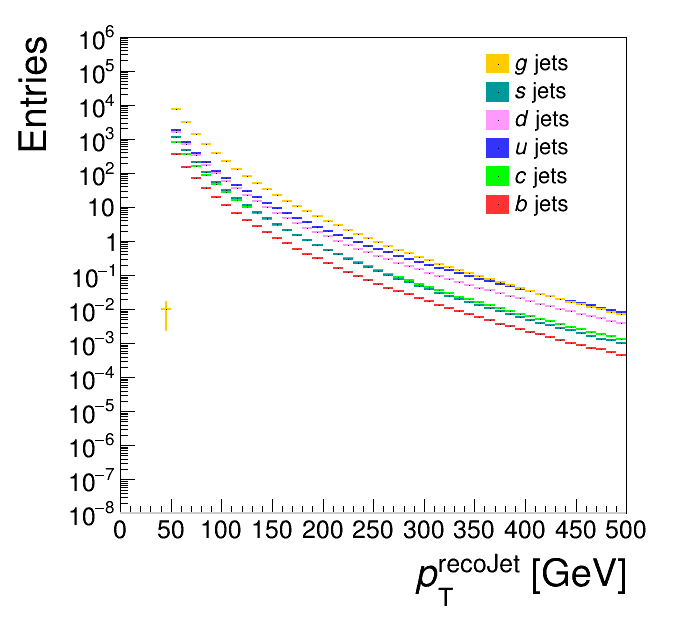
\includegraphics[width=0.8\textwidth]{flavor-spectra.png}};
    \end{tikzpicture}
    \column{0.5\textwidth}
    \begin{tikzpicture}
      \node{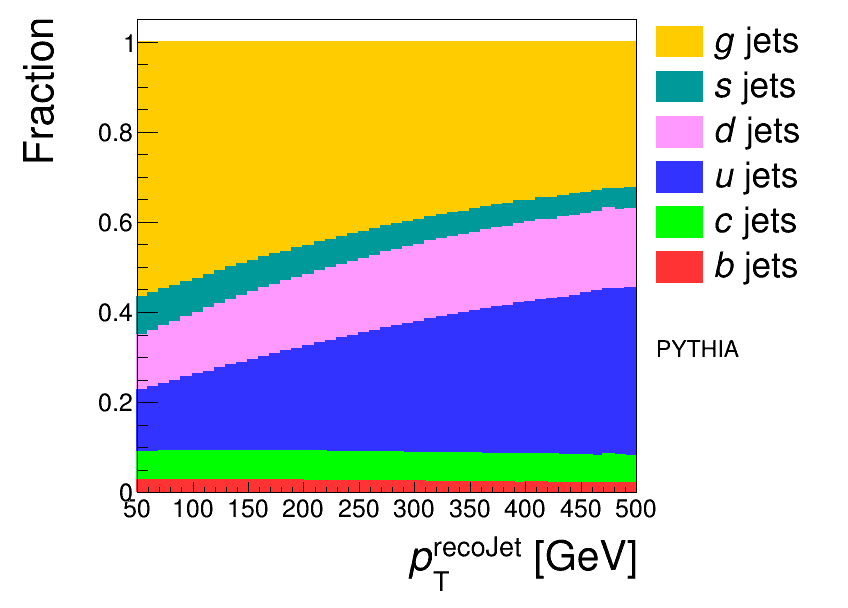
\includegraphics[width=1.0\textwidth]{flavor-fraction.png}};
    \end{tikzpicture}
  \end{columns}
\end{frame}
